\section{Produkt"ubersicht}%

\textit{Worthwhile} ist ein m"achtiges Analysewerkzeug f"ur eine einfache WHILE-""Programmiersprache. Bei der Programmanalyse kommen dabei sowohl klassische Techniken der Laufzeitanalyse (interaktives Debuggen, Überprüfung von Zusicherungen zur Laufzeit) als auch moderne, logikbasierte Methoden der Softwareverifikation zum Einsatz.\footnote{Quelle: Projektspezifikation unter \url{http://formal.iti.kit.edu/teaching/pse/2011/}} \textit{Worthwhile} vereinigt s"amtliche Arbeitsschritte von der Programmerstellung bis zur Programmverifikation unter einer einzigen komfortablen und leicht benutzbaren Oberfl"ache. Außerdem ist \textit{Worthwhile} Ausführungsumgebung für die entwickelten WHILE-""Programme.%

\subsection{Anwendungsfall-""Übersicht}

Im folgenden Anwendungsfalldiagramm sind die unterschiedlichen Möglichkeiten zur Benutzung des Systems dargestellt:

\begin{figure}[H]
	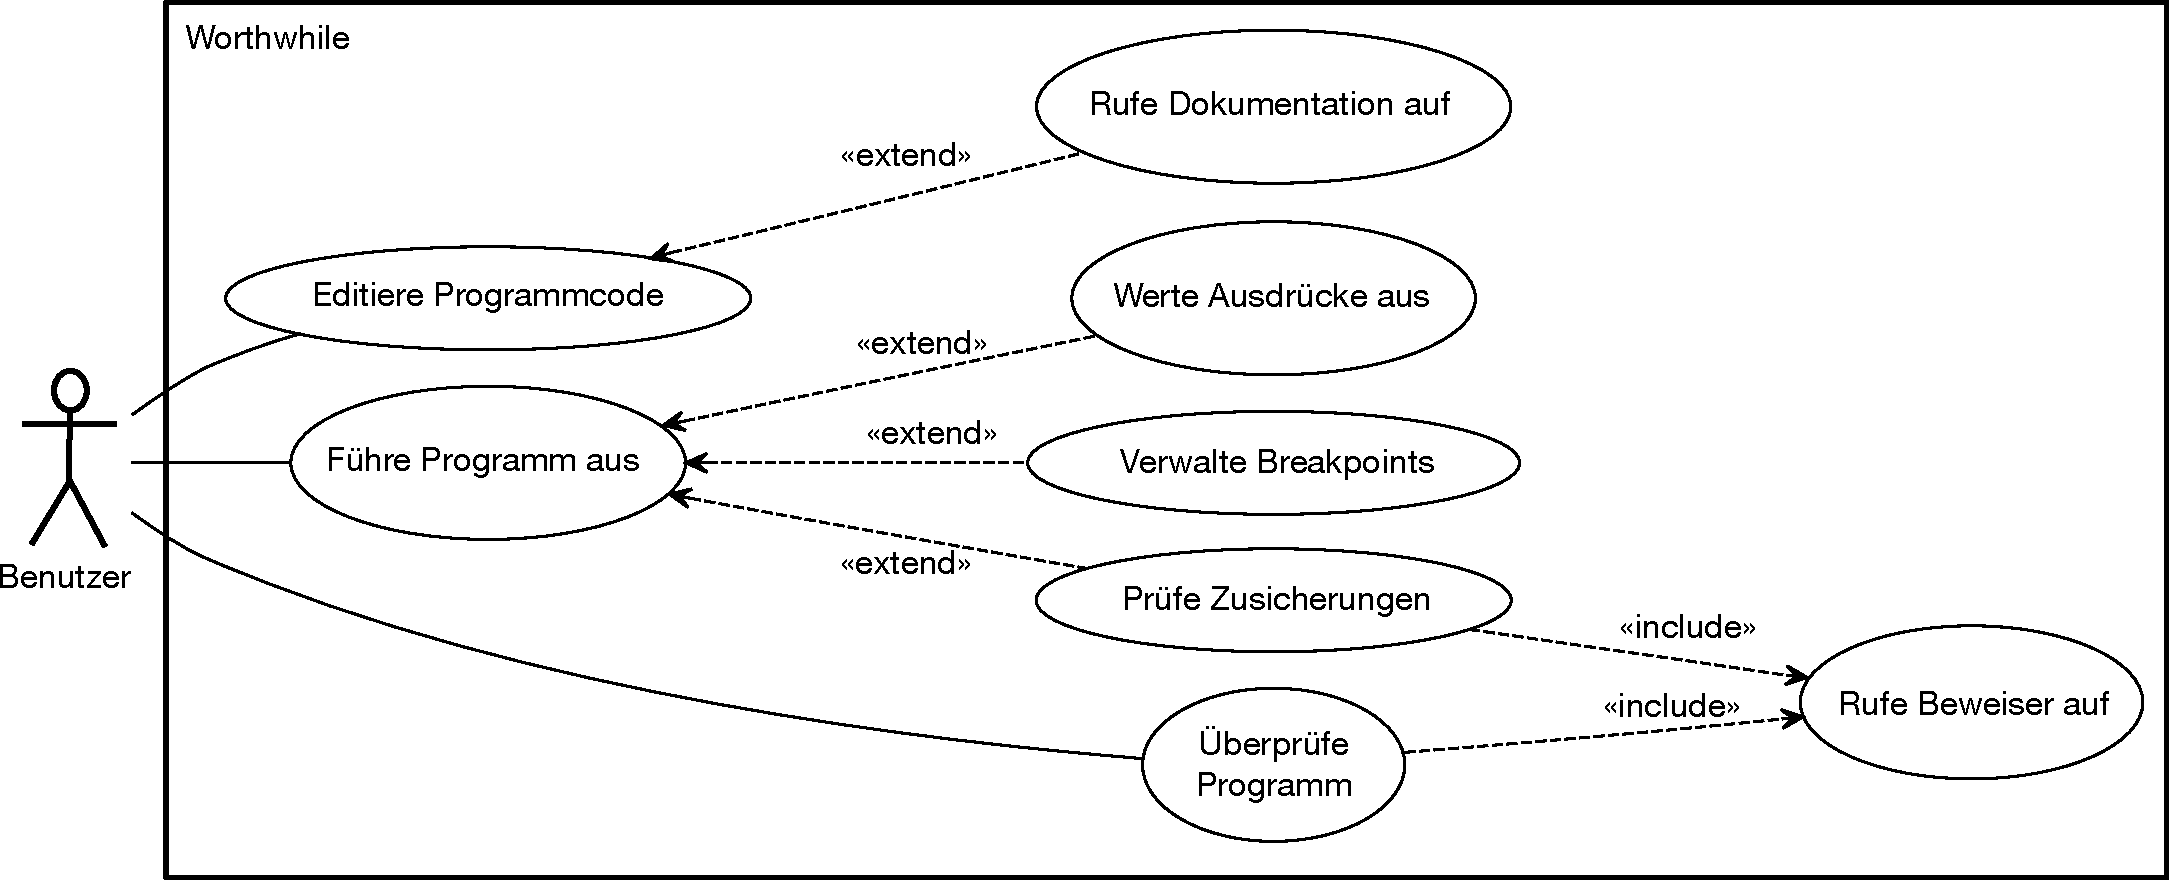
\includegraphics[width=\textwidth]{usecase/usecase.pdf}
\end{figure}
